
\begin{figure}
\centering
\begin{tikzpicture}[scale=1.6]
\draw (-2,0) -- (2,0);
\draw[dotted, smooth, domain=-2:1.7, color=blue, line width=0.15mm] 
    plot (\x,{-0.55/(\x-2)});
\draw (-2,-0.2) -- (-2,0);
\draw (2,-0.2) -- (2,0);


\def\names{{-0.1,0.2,-1.25,0.4,-0.7,-1.5}}
\def\nameh{{0.114942528735632,
0.128205128205128,
0.082304526748971,
0.138888888888889,
0.095238095238095,
0.077519379844961
}}

\foreach \x in {0,...,5} {
\draw (\names[\x],0) -- (\names[\x],\nameh[\x]*5);
\draw	(\names[\x],-0.25) node{{ $a_{\x}$}};
\draw[black,fill] (\names[\x],\nameh[\x]*5) circle (0.20mm);
}

\draw (0.8,-0.1) -- (0.8,0.1);
\draw	(0.8,-0.25) node{{ $\mu$}};

\draw (2,0) -- (2,0.3629*5);
\draw	(2.15,0.0) node{{ $a_j$}};
\draw[black,fill] (2,0.3629*5) circle (0.20mm);

\draw	(-2,-0.35) node{{ $-2$}};
\draw	(2,-0.35) node{{ $2$}};

\end{tikzpicture}
%\caption{For sample points $a_0,\dots,a_5 = \{-0.1,0.2,-1.25,0.4,-0.7,-1.5\}$ each with single multiplicity drawn from a distribution bounded between $-2$ and $2$ with a mean $\mu=0.8$, the probability of the distribution that maximises likelihood is: $0.128,0.082,0.139,0.095,0.078$ probabilities for the sampled values respectively with the probability of drawing the unsampled value $2$ being $0.363$. We also see the probabilities having hyperbolic weighting centered at $G=a_j=2$ }
\caption{For distributions bounded between -2 and 2, with a specified mean $\mu$, the distribution that maximises the likelihood of drawing sample values $a_0,\dots,a_5$ (each with single multiplicity) including the unsampled value 2. We also see the hyperbolic weighting of probabilities centered at 2.}
\label{illustration1}
\end{figure}


\begin{figure}
\centering
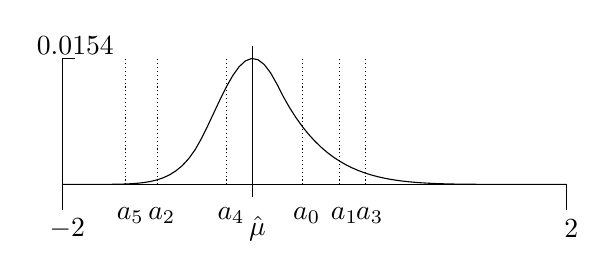
\begin{tikzpicture}[scale=1.6]
\draw (-2,0) -- (2,0);
\draw (-2,-0.2) -- (-2,1);
\draw	(-1.9,1.1) node{{$0.0154$}};
\draw (-2,1) -- (-1.9,1);
\draw (2,-0.2) -- (2,0);


\def\names{{-0.1,0.2,-1.25,0.4,-0.7,-1.5}}

\foreach \x in {0,...,5} {
\draw[densely dotted] (\names[\x],0) -- (\names[\x],1);
\draw	(\names[\x],-0.25) node{{ $a_{\x}$}};
%\draw[black,fill] (\names[\x],1) circle (0.20mm);
}

\draw	(-2,-0.35) node{{ $-2$}};
\draw	(2,-0.35) node{{ $2$}};

\draw (-0.491666,-0.1) -- (-0.491666,1.1);
\draw	(-0.491666,-0.35) node{{ $\hat{\mu}$}};

\draw (-2, 0.0) -- (-1.95, 3.1949045106940002e-09) -- (-1.9, 2.0447388868441601e-07) -- (-1.85, 2.329085388295906e-06) -- (-1.8, 1.308632887580254e-05) -- (-1.75, 4.99203829795935e-05) -- (-1.7, 0.00014906146485093864) -- (-1.65, 0.0003758773207786371) -- (-1.6, 0.0008375250480513626) -- (-1.55, 0.0016979032480677206) -- (-1.5, 0.003194904510693984) -- (-1.45, 0.0056599682298695475) -- (-1.4, 0.009539933750460073) -- (-1.35, 0.015421193846358306) -- (-1.2999999999999998, 0.024056148529832774) -- (-1.25, 0.036391959192123666) -- (-1.2, 0.0536016030752873) -- (-1.15, 0.07711722807528733) -- (-1.1, 0.10866580787633412) -- (-1.0499999999999998, 0.15030709741647255) -- (-1.0, 0.204473888684415) -- (-0.95, 0.27401456684762604) -- (-0.8999999999999999, 0.3620471567576104) -- (-0.8499999999999999, 0.46301593037110456) -- (-0.7999999999999998, 0.5694580368789878) -- (-0.75, 0.6759144001292552) -- (-0.7, 0.7762820274984882) -- (-0.6499999999999999, 0.8642853711025698) -- (-0.5999999999999999, 0.933992911725407) -- (-0.5499999999999998, 0.9803369907493318) -- (-0.5, 0.9995923847771935) -- (-0.44999999999999996, 0.9897691772744265) -- (-0.3999999999999999, 0.9508785474839102) -- (-0.34999999999999987, 0.8850363214801366) -- (-0.2999999999999998, 0.7963785080757475) -- (-0.25, 0.6985028085753533) -- (-0.19999999999999996, 0.6103924216093528) -- (-0.1499999999999999, 0.5317454806837659) -- (-0.09999999999999987, 0.4617307692307688) -- (-0.04999999999999982, 0.39957307361552535) -- (0.0, 0.3445506091008736) -- (0.050000000000000266, 0.2959925063775508) -- (0.10000000000000009, 0.2532763586599564) -- (0.1499999999999999, 0.21582582934744807) -- (0.20000000000000018, 0.1831083202511772) -- (0.25, 0.15463270038646193) -- (0.30000000000000027, 0.12994709533069307) -- (0.3500000000000001, 0.10863673714678175) -- (0.40000000000000036, 0.09032187487213929) -- (0.4500000000000002, 0.07465574557319755) -- (0.5, 0.0613226059654631) -- (0.5500000000000003, 0.050035824599109914) -- (0.6000000000000001, 0.04053603461010866) -- (0.6500000000000004, 0.032589347036891626) -- (0.7000000000000002, 0.025985624702555898) -- (0.75, 0.020536816662602042) -- (0.8000000000000003, 0.016075353218210336) -- (0.8500000000000001, 0.01245260149505354) -- (0.9000000000000004, 0.00953738158764612) -- (0.9500000000000002, 0.00721454326923076) -- (1.0, 0.00538360326720115) -- (1.0500000000000003, 0.003957443104061813) -- (1.1, 0.002861067503924644) -- (1.1500000000000004, 0.0020304233645420757) -- (1.2000000000000002, 0.0014112792948771764) -- (1.25, 0.000958165718210361) -- (1.3000000000000003, 0.0006333755407829468) -- (1.35, 0.0004060253859774359) -- (1.4000000000000004, 0.00025117739403453595) -- (1.4500000000000002, 0.00014902158730697063) -- (1.5, 8.411880105001797e-05) -- (1.5500000000000003, 4.4704179748822446e-05) -- (1.6, 2.205123898245588e-05) -- (1.6500000000000004, 9.896492824733505e-06) -- (1.7000000000000002, 3.924646781789624e-06) -- (1.75, 1.3143562664065307e-06) -- (1.8000000000000003, 3.445506091008709e-07) -- (1.85, 6.132260596546288e-08) -- (1.9000000000000004, 5.383603267201036e-09) -- (1.9500000000000002, 8.411880105001619e-11) -- (2.0, 0.0);

\end{tikzpicture}
\caption{For distributions bounded between -2 and 2 and with the same sample values $a_0,\dots,a_5$ as in figure \ref{illustration1}, the maximum probability that the mean $\mu=x$ consistant with thoes sample values per Theorem \ref{main_theorem}. We see that the maximum height is at the sample mean $\hat{\mu}$ and is very small, and we can see that there is a slightly heavier right side tail as the data samples are left heavy.}
\label{illustration2}
\end{figure}


